\documentclass[12pt]{article}
%Gummi|065|=)
\usepackage{amsmath, amsfonts, amssymb}
\usepackage[landscape, margin=0.5in]{geometry}
\usepackage{xcolor}
\usepackage{graphicx}
\newcommand{\off}[1]{}
\DeclareMathSizes{20}{30}{21}{18}

\usepackage{tikz}

\title{\textbf{ Unipotent Flows }}
\author{John D Mangual}
\date{}
\begin{document}

\fontfamily{qag}\selectfont \fontsize{25}{30}\selectfont

\maketitle

% note AVOID THE WORDS 'Ratner Theorem' instead explain what it is

\noindent 

\newpage

\noindent \textbf{The matrix $\left(\begin{array}{cc}
1 & 1 \\ 0 & 1 \end{array} \right) $ also known as $(x,y) \mapsto (x+y,y)$} \newline

\noindent Ratner's Theorem says\footnote{Somtimes in a very difficult theorem we start of great with a clear discussion with lots of illustration.  Then after some point we decide everything is ``technical" and go for dozens of pages which basically can be omitted.  This statement is due to Manfred Einsiedler, whose exposition is a simplification of a simplification of a simplification\dots The work is endless.} 

\begin{quotation}
\noindent Let $G$ be a Lie group, $\Gamma < G$ be a discrete subgroup, and $H < G$ be a subgroup isomorphic to $\mathrm{SL}(2, \mathbb{R})$.  \newline

\noindent Then any $H$-invariant and ergodic probability measure $\mu$ on $X = \Gamma \backslash G$ is homogeneous.  \newline

\noindent i.e. there is \begin{itemize}
\item a closed connected subgroup $L < G$ containing $H$ such that $\mu$ is $L$-invariant and 
\item some $x_0 \in X$ such the $L$-orbit $x_0L$ is closed and supports $\mu$
\end{itemize}
That means $\mu$ is an $L$-invariant volume measure on $x_0L$
\end{quotation}

\newpage

\noindent \textbf{Why Learn Ratner's Theorem?} \newline

\noindent There are integers $(a,b,c)$ such that $|a^2 + b^2 - \sqrt{2}c^2 |< \epsilon$ \newline
Why can this have arbitrarily small numbers? This is proven by Dani and Margulis\footnote{ Although I find a closed proof of Bourgain of certain cases in 2016}
\newline

\noindent Ratner's Theorem on the equidistribution of the horocycle flow seems to do with the shear of a rhombus.
\newline


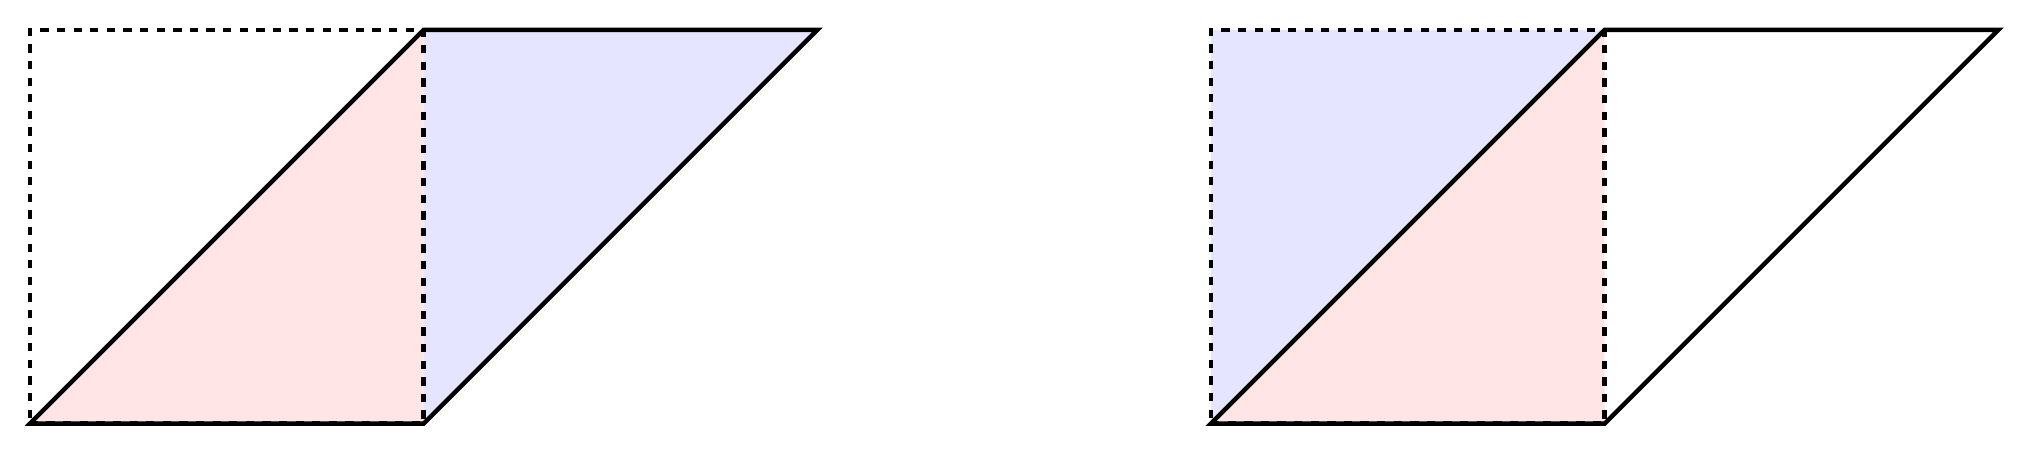
\begin{tikzpicture}

\path[fill=red!10!white] (0,0)--(5,0)--(5,5)--cycle;

\path[fill=blue!10!white] (5,0)--(10,5)--(5,5)--cycle;

%\path[fill=blue!10!white] (0,0)--(5,5)--(0,5)--cycle;

\draw[ultra thick, dashed] (0,0)--(5,0)--(5,5)--(0,5)--cycle;
\draw[ultra thick] (0,0)--(5,0)--(10,5)--(5,5)--cycle;

\begin{scope}[xshift=15cm]

\path[fill=red!10!white] (0,0)--(5,0)--(5,5)--cycle;

%\path[fill=blue!10!white] (5,0)--(10,5)--(5,5)--cycle;

\path[fill=blue!10!white] (0,0)--(5,5)--(0,5)--cycle;

\draw[ultra thick, dashed] (0,0)--(5,0)--(5,5)--(0,5)--cycle;
\draw[ultra thick] (0,0)--(5,0)--(10,5)--(5,5)--cycle;

\end{scope}
\end{tikzpicture}

This in turn has to do with Euclid's Elements.  The shear preserves area, these two rectangles have equal area.  Just take a pair of scissors and cut.

\newpage

\noindent Our goal is to try to express some of these ``entropy" considerations in simple language.  And I need to re-write all of these statements since I am not an expert on Ratner Theorem.


\newpage

\noindent \textbf{Instances of $(x,y) \to (x+y,y)$ in number theory} \\ \\
In one paper I found an isomorphism from $\text{PGL}_2$ to $\text{SO}_3$:

$$ \left[\begin{array}{cc}
a & b \\ c & d \end{array} \right] \mapsto (ad-bc)^{-1}
\left[ \begin{array}{ccc} 
ad + bc & i(ac+bd) & bd-ac \\
-i(ab+cd) & \frac{a^2 + b^2 + c^2 + d^2}{2}
& i \frac{a^2 - b^2 + c^2 - d^2}{2} \\ 
-(ab-cd) & i \frac{-a^2 - b^2 + c^2 + d^2}{2} & 
\frac{a^2 - b^2 - c^2 + d^2}{2} \end{array}\right]$$
Over which field is this an isomorphism?  Certainly not $\text{PGL}_2(\mathbb{R}) \not \simeq \text{SO}_3(\mathbb{R}).$  Instead\footnote{The source I am reading has $k$ to be a field of characteristic $0$ and $k^s$ is a fixed separable closer.  So if $k = \mathbb{Q}$ the fractions, and $k^s \subset \overline{\mathbb{Q}}$ are the separable elements of the algebraic closure.  This is a humungous field instead I pick anything with $\mathbb{Q}(\sqrt{2}, i) = \mathbb{Q}[x,y]/(x^2 - 2, y^2 + 1)$} we could try the $p$-adic numbers $ \mathbb{Q}_p = \stackrel{\lim}{\to} \mathbb{Q}[\frac{1}{p^k}] $ (did I type that correctly?) What if I plug in $a = b = d = 1$ and $c = 0$ ?

$$ \left[\begin{array}{cc}
1 & 1 \\ 0 & 1 \end{array} \right] \mapsto 
\left[ \begin{array}{rrr} 
1 & i & 1 \\
-i & \frac{3}{2}
&  -\frac{i}{2} \\ 
-1 &  \frac{i}{2} & 
\frac{1}{2} \end{array}\right]$$
$\sqrt{-1} \in \mathbb{Q}_5$ and $\sqrt{-1}\notin \mathbb{Q}_3$ but there is still an isomorphism.
\newpage


\noindent \textbf{Instances of $(x,y) \to (x+y,y)$ in number theory} \\ \\
This wedge product notation is rather modern, instead of determinants:
$$ \xi \mapsto 1 \wedge \xi \wedge \xi^2 : C / A \to \wedge^3 C $$
This is a map from a cubic ring modulo a principal ideal domain\footnote{For example $C = \mathbb{Z}[e^{2\pi i / 3}]= \mathbb{Z}\cdot 1 \oplus \mathbb{Z} \cdot e^{2\pi i / 3} \oplus \mathbb{Z}\cdot e^{4\pi i / 3}$ and $A = \mathbb{Z}$}.  If 
$$ \phi(x,y) = ax^3 + bx^2 y + c xy^2 + dy^3$$
with the $\text{GL}_2(A)$ action:
$$ \left(\left[ 
\begin{array}{cc} p & q \\ r & s\end{array}
\right], \phi \right)(x,y) = \frac{1}{ps-qr}\phi(px + ry, qx + sy) $$
so if I plug in $p=q=s=1$ and $r = 0$:
$$ a(x+ty)^3 + b(x+ty)^2 y + c(x+ty)y^2 + dy^3 $$
is a unipotent flow on the space of cubic forms.
$$ a\,x^3 + (3at+b)\,x^2 y + (3at^2 + 2bt + c)\,xy^2 + (at^3 + bt^2 + ct + d)\,y^3 $$
and each coefficients is the derivative of the one after.
\newpage

\noindent \textbf{Mixing of $(x,y) \to (x+y,y)$ in Number Theory} \\ \\
Both flows I have shown on the previous page are \textit{mixing}.  How mixing can adding $x + ty$ be?  How do we quantify the mixiness of adding $+1$?

\newpage

\fontfamily{qag}\selectfont \fontsize{12}{10}\selectfont

\begin{thebibliography}{}

\item Evan M. O'Dorney	 \textbf{A remarkable identity in class numbers of cubic rings.} \texttt{arXiv:1608.00166}

\item Jack A. Thorne \textbf{Arithmetic invariant theory and 2-descent for plane quartic curves} \texttt{arXiv:1607.08816}

\item Manjul Bhargava \textbf{Higher composition laws II: On cubic analogues of Gauss composition} \\  \texttt{http://annals.math.princeton.edu/2004/159-2/p09}

\item Manjul Bhargava \textbf{The density of discriminants of quintic rings and fields}  
\texttt{arXiv:1005.5578}


\end{thebibliography}


\end{document}

